% parametros del documento
\documentclass[11pt,a4paper]{article}
\usepackage[margin=2cm, top=3cm, includefoot]{geometry} 

% importacion de modulos necesarios
\usepackage[utf8]{inputenc} % codificacion UTF-8
\usepackage[spanish]{babel} % para el idioma español
\usepackage[parfill]{parskip} % para ajustar el espaciado
\usepackage[hidelinks]{hyperref} % para la insercion de links
\usepackage{fancyvrb} % para el uso de formatos personalizados
\usepackage{listings} % para la insercion de código fuente
\usepackage{xcolor} % para ña insercion de colores
\usepackage{graphicx} % para la insercion de imagenes
\usepackage{fancyhdr} % para el ajuste de las cabeceras

% importacion de modulos externos 
newcommand{gitversion}{ae26833}
newcommand{gitdate}{2024-07-12}
newcommand{gitcreated}{2024-07-12}
 % para la obtencion de los datos de control

% definicion de variables de color
\definecolor{codegreen}{rgb}{0,0.6,0}
\definecolor{codegray}{rgb}{0.5,0.5,0.5}
\definecolor{codepurple}{rgb}{0.58,0,0.82}
\definecolor{backcolour}{rgb}{0.95,0.95,0.92}
\definecolor{background}{HTML}{dbdbdb}

% definicion de variables de imagenes
\newcommand{\enterpriselogo}{images/colnex.png}

% definicion del formato de las inserciones de codigo
\lstdefinestyle{mystyle}{
    backgroundcolor=\color{backcolour},   
    commentstyle=\color{codegreen},
    keywordstyle=\color{magenta},
    numberstyle=\tiny\color{codegray},
    stringstyle=\color{codepurple},
    basicstyle=\ttfamily\footnotesize,
    breakatwhitespace=false,         
    breaklines=true,                 
    captionpos=b,                    
    keepspaces=true,                 
    numbers=left,                    
    numbersep=5pt,                  
    showspaces=false,                
    showstringspaces=false,
    showtabs=false,                  
    tabsize=2
}
\lstset{style=mystyle}

% cambio de nombre para la tabla de contenidos
\addto\captionsspanish{\renewcommand{\contentsname}{Índice de Contenidos}}

% definicion del formato de la cabecera
\setlength{\headheight}{50pt}
\pagestyle{fancy}
\fancyhf{}
\rhead{\includegraphics[width=3cm]{\enterpriselogo}}
\renewcommand{\headrule}{\hbox to\headwidth{\color{background}\leaders\hrule height \headrulewidth\hfill}}

% inicio del documento
\begin{document}

% portada
\begin{titlepage}
    \centering
    \includegraphics[width=0.4\textwidth]{\enterpriselogo}
    \par
    \vfill
    {\LARGE\bfseries Walkthrough}
    \par\vspace{0.5cm}
    {\Large\bfseries Montaje del servicio de Front-End con Docker}
    \vfill
    \begin{flushright}
        {\large {\bfseries Fecha de Creación:} \gitcreated}\par\vspace{0.2cm}
        {\large {\bfseries Última Actualización:} \gitdate{}}\par\vspace{0.3cm}
        {\large {\bfseries Versión del Documento:} \gitversion{}}
    \end{flushright}
  \vfill
  Este documento es confidencial.
  No debe ser impreso, divulgado o compartido con terceros.
\end{titlepage}

% tabla de contenidos
\pagenumbering{Roman}
\tableofcontents
\newpage
\pagenumbering{arabic}

% inicio de contenidos

\section{Introducción}
Este documento pretende explicar de manera detallada el proceso requerido para la descarga,
instalación y montaje del servicio de Front-End a partir de Docker.\par
Dentro del alcance de estos desarrollos se incluyen todos los colaboradores asociados al
desarrollo del programa de reporte de actividades de Colnex SI en el campo de la programación web.

\section{Descarga de la imagen de Docker}
El primer paso es adquirir la imagen desde la url en que se aloja:\par
\textit{https://drive.usercontent.google.com/download?id=1A\_FAfXEvndUtWB6G6i58qo3OV4jJt-Mq}\par
Para ello, podemos usar el comando \textit{curl} o la instrucción \textit{wget}
de la siguiente manera.

\begin{figure}[h]
    \begin{lstlisting}[language=Bash]
        // Comando para descargar la imagen con Wget
        wget --load-cookies /tmp/cookies.txt "url"

        // Comando para descargar la imagen con cURL
        curl -L -o frontend.tar.gz "url"
    \end{lstlisting}
\end{figure}

Adicionalmente, usted puede utilizar el recurso de la siguiente URL para descargar la imagen:\par
\centerline{\textit{\href{https://github.com/chentinghao/download_google_drive}{chentinghao/download\_google\_drive}}}

\vspace{5cm}

\section{Comprobación de la integridad del archivo}
Para verificar que el archivo que contiene la imagen de Docker se ha descargado de manera original 
y sin ninguna alteración, es una buena práctica contar con un hash que permita validar esto y comparar
que el que se genera con la copia descargada sea idéntico al original.\par

\begin{figure}[h]
    \begin{lstlisting}[language=Bash]
        // Hash original
        39BA72736A803089C15941B7C6C0249C
    \end{lstlisting}
\end{figure}

\begin{figure}[h]
    \begin{lstlisting}[language=Bash]
        // Comando para obtener el hash en Windows Powershell
        Get-FileHash frontend.tar.gz -Algorithm MD5

        // Comando para obtener el hash en Linux
        md5sum frontend.tar.gz
    \end{lstlisting}
\end{figure}

\newpage

\section{Montaje de la imagen de Docker}
Para instalar e iniciar la imagen Docker, es necesario ejecutar estos comandos:

\begin{figure}[h]
    \begin{lstlisting}[language=Bash]
        // Comando para importar la imagen de docker
        docker import frontend.tar.gz frontend:frontend

        // Comando para ejecutar la imagen de docker
        docker run -d -p 8090:80 --name "Frontend" -it frontend nginx -g "daemon off;"
    \end{lstlisting}
\end{figure}

\section{Notas de ejecución}
Normalmente el comando anteriormente utilizado para iniciar la imagen de Docker 
genera un error al no encontrar la imagen o contenedor \textit{frontend} por lo que, 
en su lugar, debemos seguir los siguientes pasos:\par

\subsection{Copiaremos el ID que aparece debajo del nombre de nuestra imagen en Docker Desktop}
\begin{figure}[h]
    \centerline{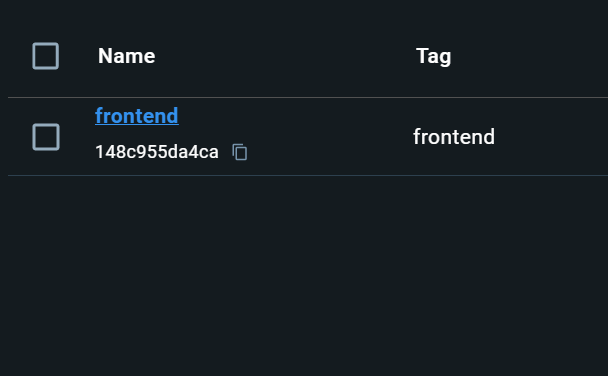
\includegraphics{images/img001.png}}
\end{figure}

\par
De no disponer de Docker Desktop, podremos obtener este identificador
al ejecutar el siguiente comando para posteriormente copiar el image ID:

\begin{figure}[h]
    \begin{lstlisting}[language=Bash]
        PS C:> docker images
        REPOSITORY   TAG        IMAGE ID       CREATED          SIZE
        frontend     frontend   148c955da4ca   55 minutes ago   195MB
    \end{lstlisting}
\end{figure}

\newpage

\subsection{Reemplazaremos la etiqueta frontend por el ID obtenido}

\begin{figure}[h]
    \begin{lstlisting}[language=Bash]
        // ejecutamos 148c955da4ca
        docker run -d -p 8090:80 --name "Frontend" -it 148c955da4ca nginx -g "daemon off;"
    \end{lstlisting}
\end{figure}

% final de contenidos y del documento
\end{document}